\section{ATLAS探测器} \label{sec:ATLAS}
ATLAS探测器座落在LHC储存环,它有25米高,44米长,总重大约7000吨。ATLAS探测器内层是内部径迹探测器(ID),其被直径为2.3米的超导螺线管包围,该超导线圈提供平行于
束流方向,大小为2 T的磁场;紧挨着ID是量能器系统,包括电磁量能器(EM)和强子量能器(HCal);最外层是$\mu$子探测器(MS)。本章将论述图~\ref{fig:ATLAS_schematic}所示的各个部分。

\begin{figure}[h]
\begin{center}
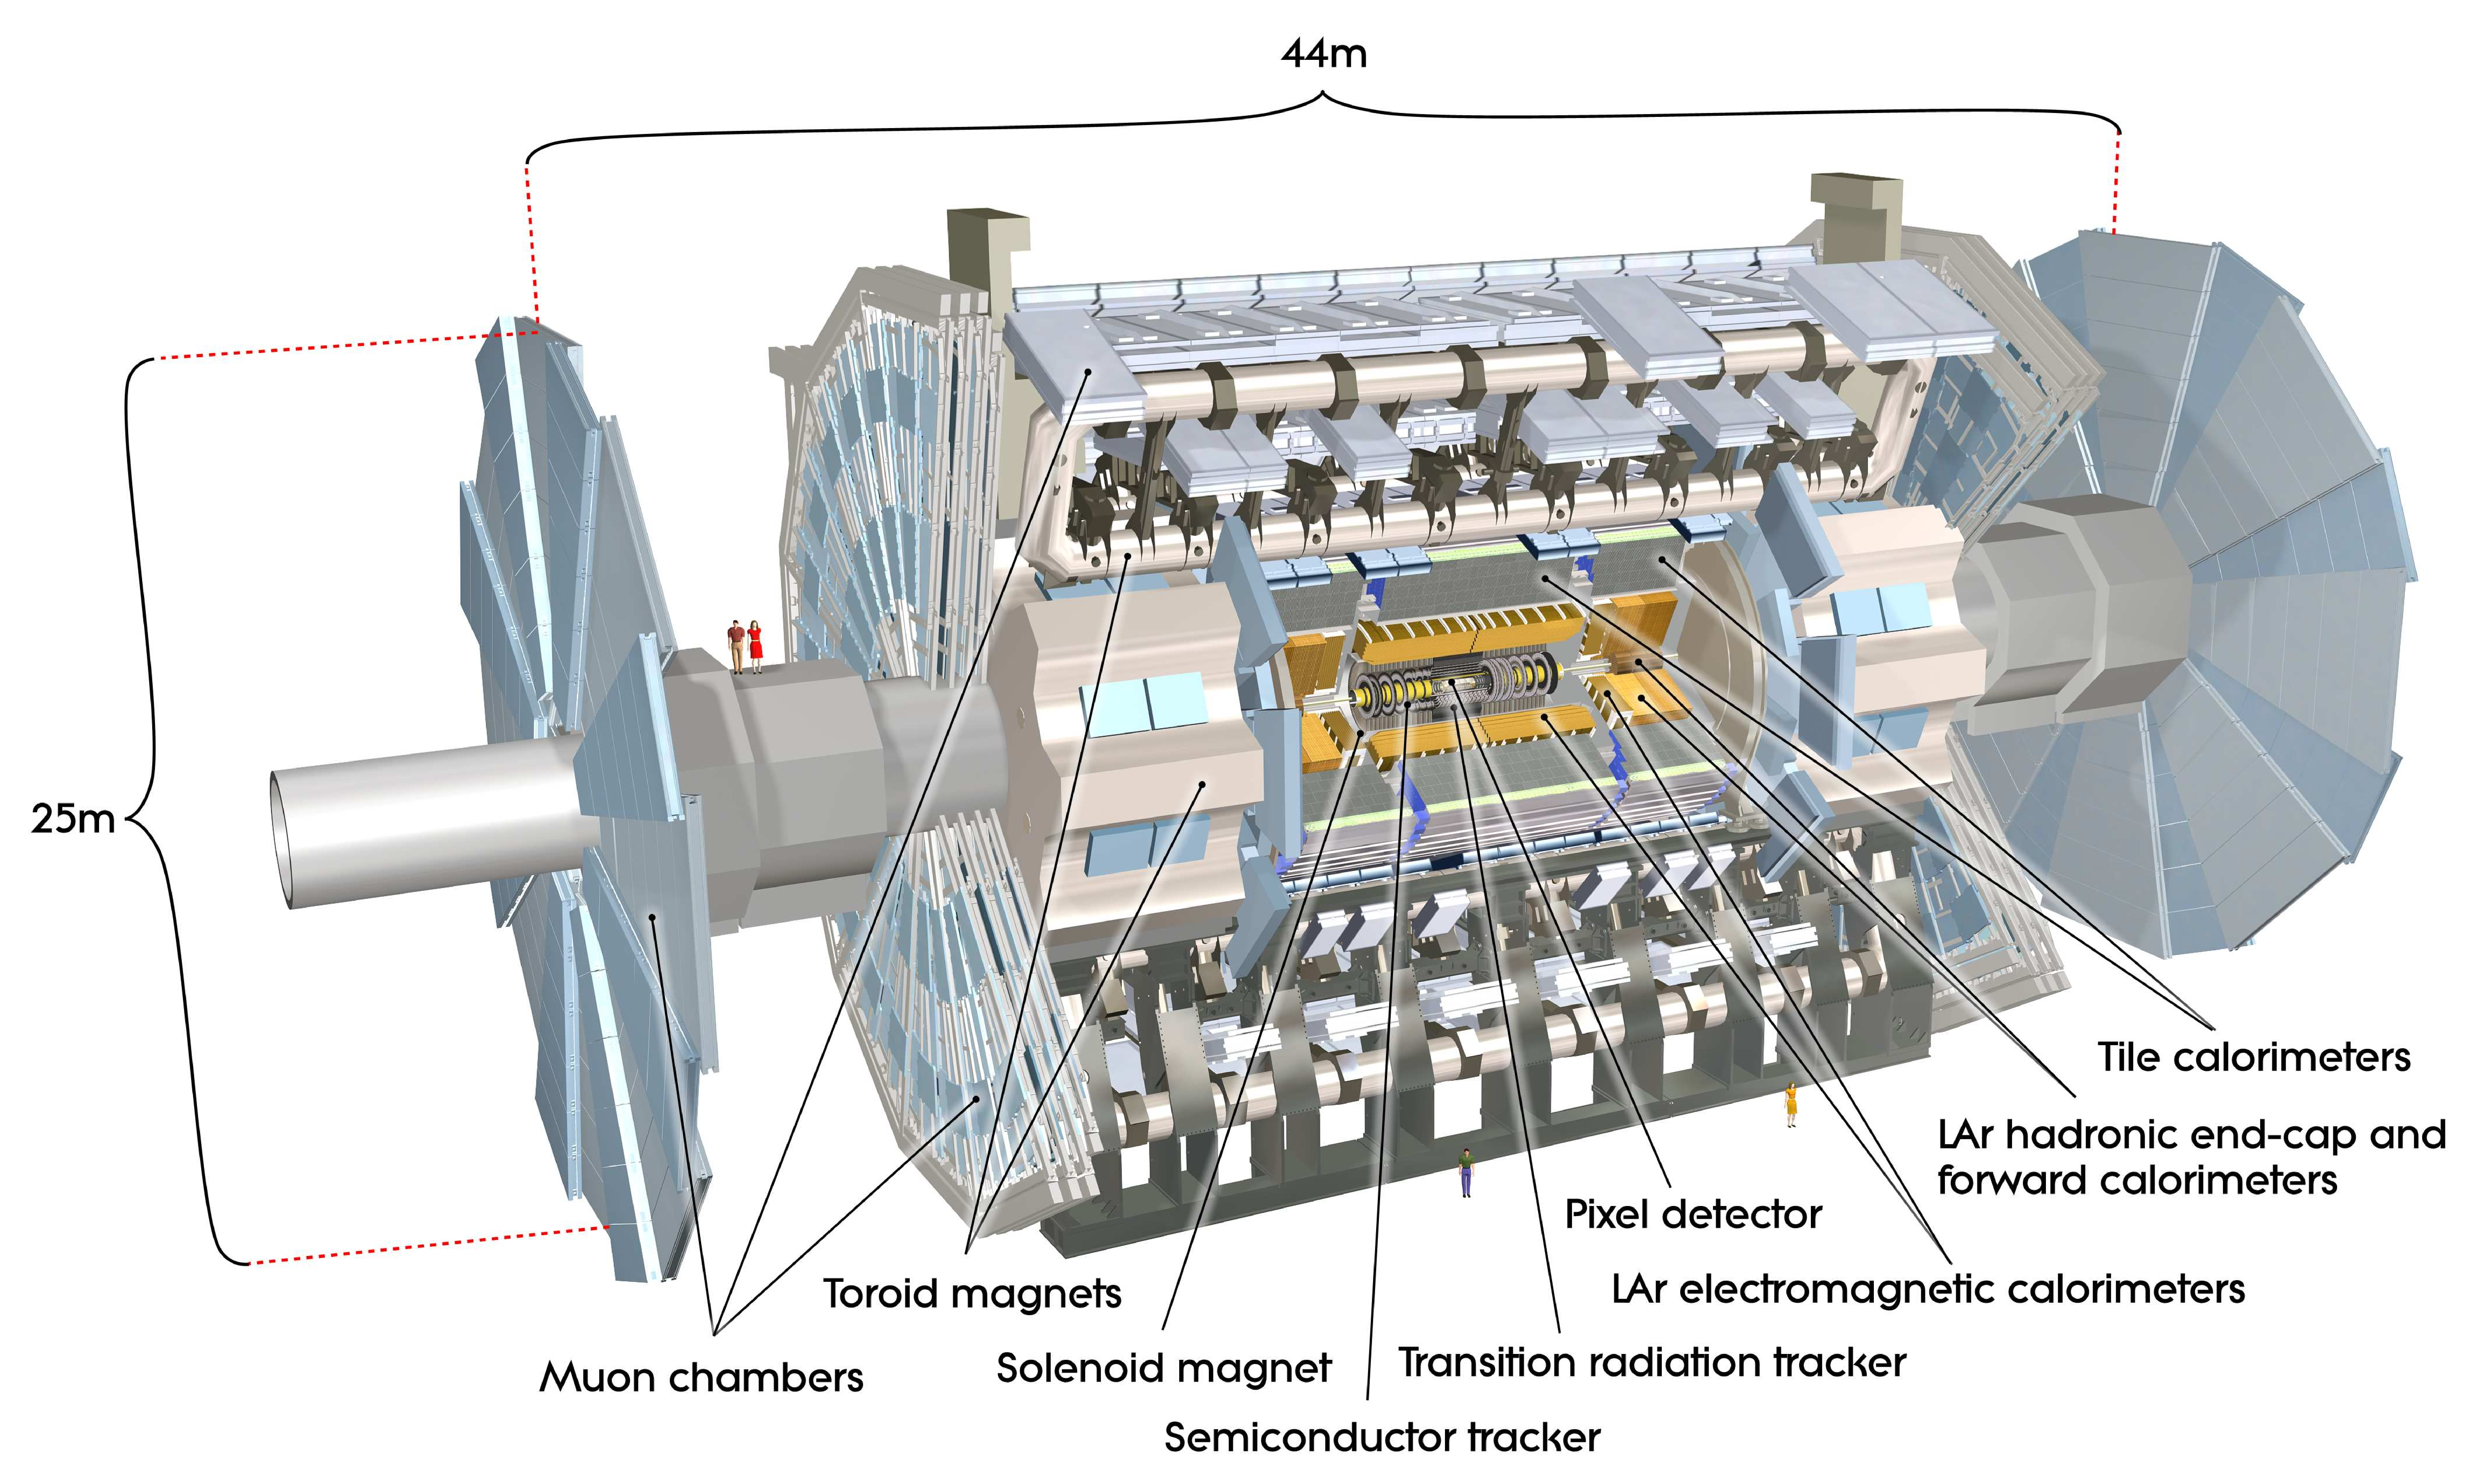
\includegraphics[width=0.9\textwidth]{fig/ATLAS_SE_Corrected7.pdf}
\caption{ATLAS探测器简图} \label{fig:ATLAS_schematic}
\end{center}
\end{figure}

\subsection{坐标系统}
ATLAS使用右手坐标系,其定义对撞点(IP)为原点,z轴为束流方向,正x轴指向环中心,正y轴则向上。在极角坐标系中,定义方位角$\phi$在(x, y)平面,大小从$-\pi$到$\pi$,极角$\theta$
从0到$\pi$,$\theta=0$时与正z轴同向。\\
赝快度定义为$\eta = -ln\tan(\theta/2)$,更大的$|\eta|$意味着粒子更靠近束流方向,在ATLAS一般称为更前向。
定义两个粒子的角距离$\Delta R=\sqrt{(\Delta\eta)^2+(\Delta\phi)^2}$。

\subsection{内部径迹探测器}
ATLAS内部径迹探测器主要用来精确寻迹(\pt > 0.1 GeV),可覆盖$|\eta|<2.5$。它包括三个子探测器,离束流中心距离从3.3 cm到101.6 cm,图~\ref{fig:ATLAS_ID_sideview}展示ID的
各个部分的分布。ID沉浸在通过铌钛超导螺线管产生的2 T轴向磁场中,线圈通过液氦冷却,温度为4.5 K。ID的强磁场可偏转带电粒子,通过测量径迹曲率可推出粒子动量。
\begin{figure}[h]
\begin{center}
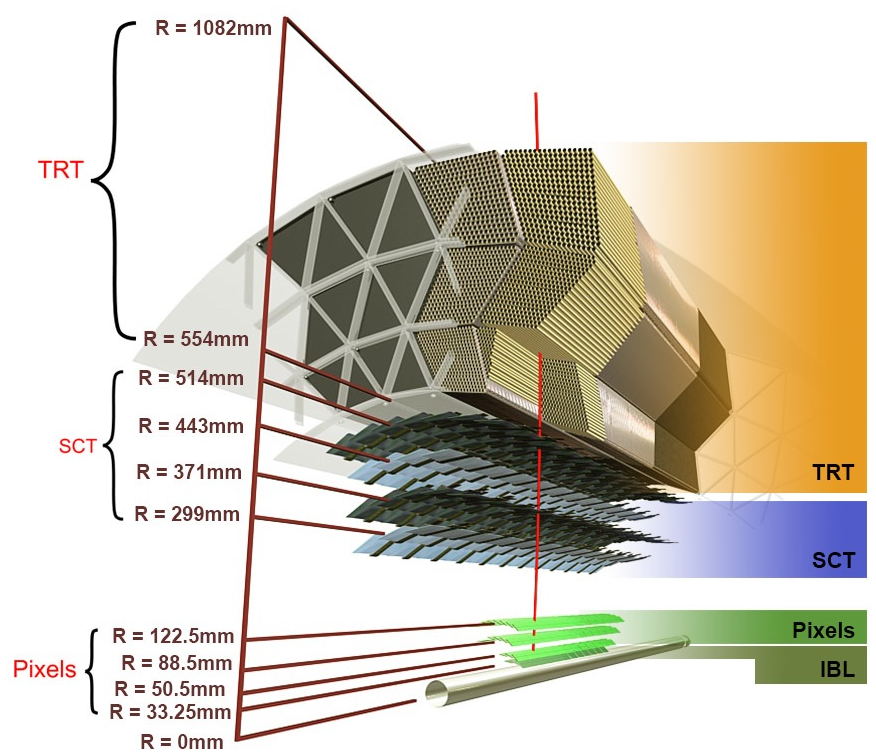
\includegraphics[width=0.9\textwidth]{fig/ATLAS_ID_sideview.png}
\caption{ATLAS内部径迹探测器} \label{fig:ATLAS_ID_sideview}
\end{center}
\end{figure}

%\subsection{像素探测器和IBL}
像素探测器(Pixel detector)围绕着束流中心,是离束流最近的系统,会经受最高密度的粒子束流,因此在ATLAS所有子探测器中具有最高的分辨率。Pixel在桶部区有四层,由1744个模块组成(module),端盖区有三层,含有288个模块。桶部区的最内层(IBL)在Run 1和Run 2之间安装,主要用于提高\bjet 鉴别。每个Pixel模块含有46080个电子学读出道,Pixel探测器总共有8千万读出道。
每个模块大小为$50\times400 \mu ~\text{m}^{2}$(IBL模块为$50\times250 \mu ~\text{m}^{2}$),其位置分辨率可达10 $\mu m$(r-$\phi$)和115 $\mu m$(z方向)。

硅微条探测器(SCT)桶部区有四层,端盖区有9层。每个SCT模块只能提供一维位置信息,所以每层SCT两个模块背靠背以一定角度粘贴在一起,加上模块本身所在位置即可
提供三维位置信息。一般SCT的分辨率为17 $\mu m$(r-$\phi$),580 $\mu m$(z方向)。SCT的总读出电子学道为630万。

穿越辐射探测器(Transition Radiation Tracker,称TRT)由大约30万,直径为4 mm充满70\%氙气,20\% CF$_4$,10\%二氧化碳的漂移管组成,桶部区的漂移管与轴线平行,端部区的漂移管
则成辐射状,其总的电子学读出道达35万。带电粒子穿过漂移管电离气体,电离电子在电压作用下达到管中心丝。桶部区(端部)只提供$r-\phi$(r-z)方向的位置测量,每条管的位置分辨率为130 $\mu\text{m}$。
TRT管层含有聚丙烯纤维和箔层,带电粒子穿过它们的边界时发射X射线,
其强度与入射粒子能量成正比,X射线通过光电效应能够产生比电离电子幅度更大的信号。
%通过这种X射线在吸管气体中的光电效应产生的电子产生的信号具有比源自经过的颗粒的信号更高的振幅。 
入射电子动量接近1 GeV时即产生明显的穿越辐射,而$\pi$介子在$\mathcal{O(100)}$~GeV动量时才产生辐射,
这可有助于粒子鉴别。

ID可为粒子径迹重建提供36个着火点($\abseta < 2.0$)。联合这三个子探测器的信息,ID可测量\pt 低至400 MeV的带电粒子,
其相应的动量分辨率可由如下公式~\cite{ATLAS_Collaboration_2008}描述:
\begin{equation}
 \frac{\sigma_{\pt}}{\pt}=0.05\%\pt\oplus1\%
\end{equation}

\subsection{量能器}
ATLAS量能系统~\cite{ATLAS_Collaboration_2008}包括几个具有不同技术和粒度的组件,涵盖非常大的范围(\abseta <4.9)。 所有组件都是采样式取数,带有吸收材料,入射粒子经过产生电磁或强子簇射,这些簇射能量仅有一部分被灵敏层检测。 量能器会利用测试束流以及探测器模拟~\cite{4436305,Davidek_2009}进行刻度,并在碰撞数据中刻度。 
ATLAS量能器的布局如图~\ref{fig:Calorimeter_d3}所示。
\begin{figure}[h]
\begin{center}
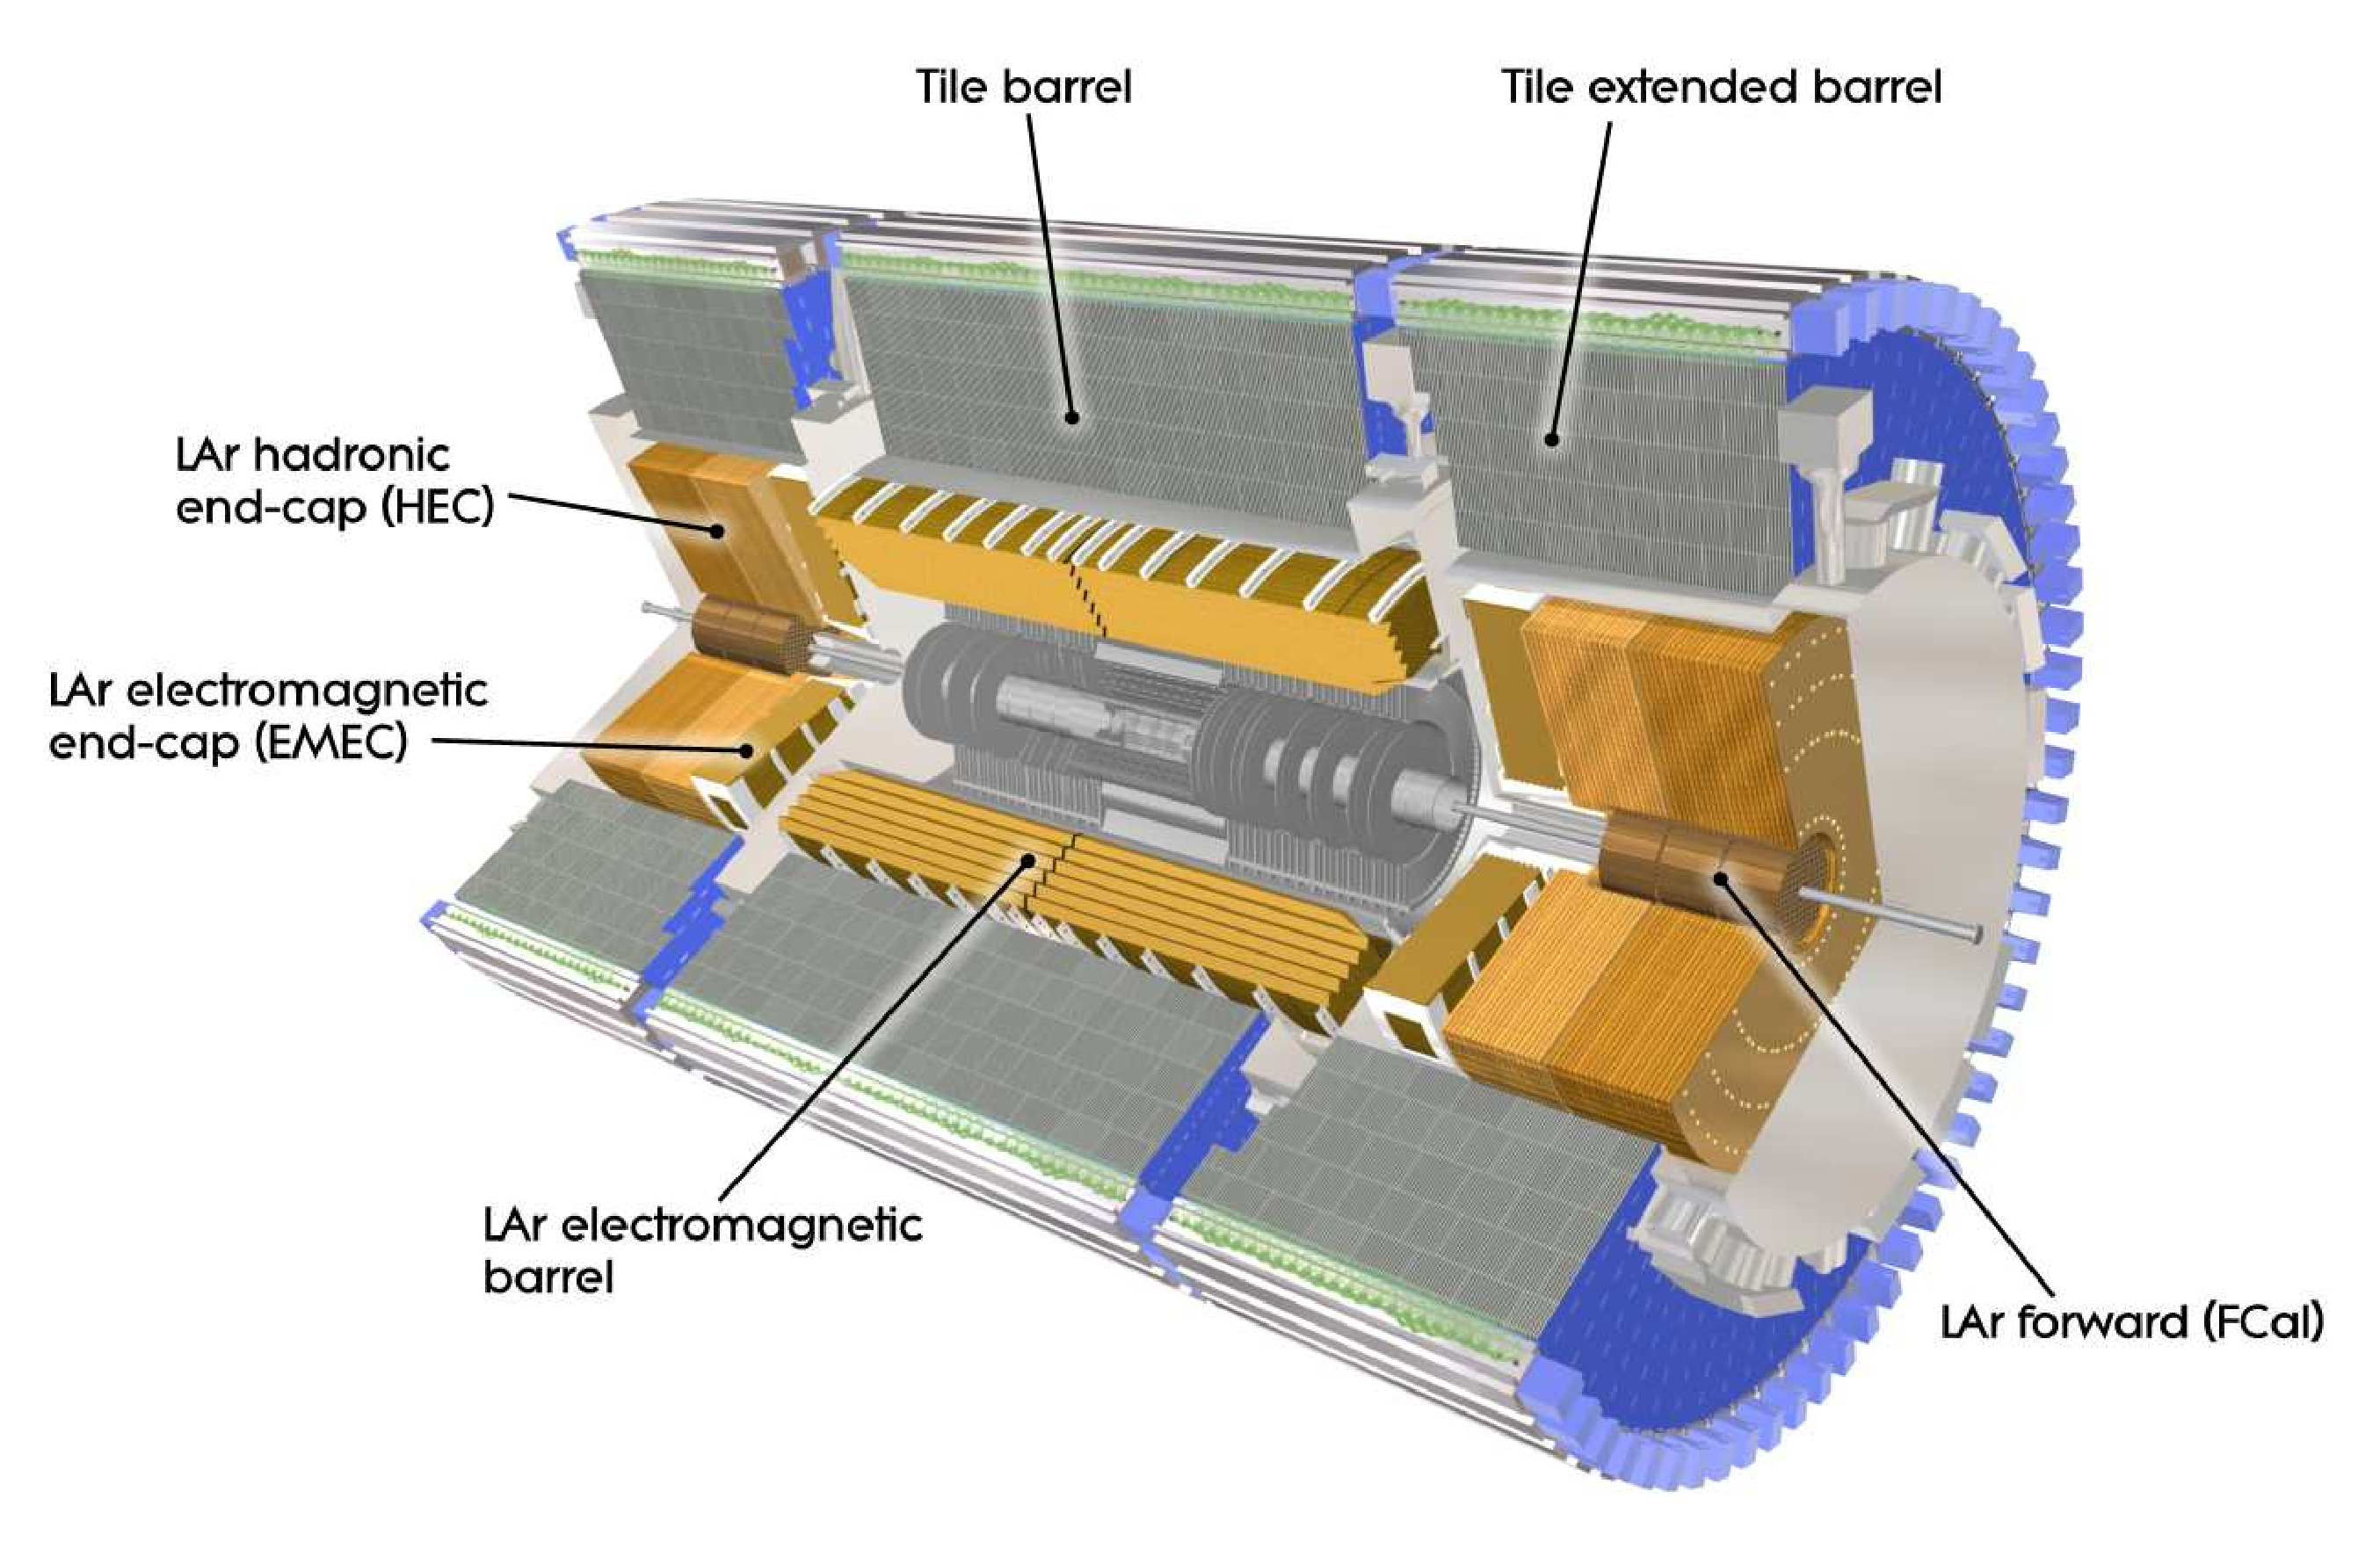
\includegraphics[width=0.9\textwidth]{fig/Calorimeter_d3.pdf}
\caption{ATLAS量能器布局} \label{fig:Calorimeter_d3}
\end{center}
\end{figure}

螺线管外部最里面的部分是电磁量能器,专门用于电子和光子的能量测量。它使用液氩(LAr)作为活性介质,具有优异的抗辐射性和能量分辨率,并容易产生电磁簇射。
读出单元是分成条状的电镀铜板电极。
EM桶部可覆盖到\abseta = 1.4,端盖系统延伸到\abseta = 3.2。
它分为3-4层,具有类似手风琴的几何形状,可提供完整的$\phi$覆盖,没有死区,并且在ID探测范围内(\abseta <2.5)具有精细的$\Delta \eta\times\Delta\phi$分辨,最小值为0.025$\times$0.025,可以分辨$\pi0\rightarrow \gamma\gamma$。
为了确保能够接收绝大数的电磁簇射,EM桶部厚度大于22个辐射长度(X0),端盖则大于24倍X0。
大多数服务设施都位于过渡区域,即$1.37<\abseta<1.52$。
%,能量测量部分缺乏,会有较差的能量测量表现。
EM能量分辨率可描述为~\cite{ATLAS_Collaboration_2008}:
\begin{equation}
\frac{\sigma_{E}}{E}=\frac{10\%}{\sqrt{E}}\oplus0.7\%
\end{equation}

强子量能器包围着电磁量能器,专门用于测量$\pi$介子和中子等强子的能量。 桶区$\abseta<1.7$由三层钢-塑料闪烁体采样量能仪(TileCal)组成,其在$\eta = 0$时总厚度为9.7倍相互作用长度($\lambda$),
以最大限度地减少强子簇射穿透HCal并到达外部$\mu$子光谱仪(punch-through)。
强子端盖量能器(HEC)覆盖$1.5<\abseta<3.2$,虽然使用铜作为被动材料并为平面状,但是与HCal采用相同的液态氩技术。
强子量能器的粒度比EM更粗,为$\Delta \eta\times\Delta\phi$为$0.1\times0.1$,
并且由于强子与材料核相互作用的性质,能量分辨率更差~\cite{ATLAS_Collaboration_2008}:
\begin{equation}
\frac{\sigma_{E}}{E}=\frac{50\%}{\sqrt{E}}\oplus3\%
\end{equation}

最后,3层前向量能计(FCal)覆盖$3.1<\abseta<4.9$以测量丢失横向能量和前向喷注。它也采用LAr技术,利用铜和钨分别作为第一层和最后两层的吸收材料。

\subsection{$\mu$子谱仪}
$\mu$子谱仪(MS)环绕着量能器,是ATLAS最外层的子探测系统,用于测量穿过ID和量能器的$\mu$子动量和位置。 MS系统有大约100万个电子学读出道,从半径5米延伸到10米,在\abseta =0处因为服务电缆有一个小间隙。
MS桶区由3个同心圆柱体组成,设计用于测量动量高于5 GeV的$\mu$子,其分辨率在100 GeV时为3\%。 端盖区有四个轮状部分,覆盖到$\abseta<2.7$。与ID类似,MS也可测量$\mu$子动量,
其磁场由大型空心环形磁体系统提供,大小在0.5~T和1~T之间。

$\mu$子室有两组系统:一组用于$\mu$子轨道的精确测量,第二组用于$\mu$子触发。精密腔室包括监测漂移管(MDT)\cite{Bauer:2016gyg}和阴极条带室(CSC)\cite{Argyropoulos:2009zz}。MDT涵盖$\abseta<2.7$的大部分区域,
 除了端盖最内层安装CSC区域$2.0<\abseta<2.7$。
 MDT由3cm直径的漂移管组成,其含有93\%氩和7\%CO$_{2}$的混合物。每根管具有单根钨-铼线,其在3kV的电压下操作,基于入射粒子产生的电离电荷的漂移时间可测量其相对位置。单管的典型空间分辨率低于100 $\mu\text{m}$,联合多层管可提升至约50~$\mu\text{m}$。

CSC由具有正交平面阴极的多丝比例室组成。它们可以处理更高的粒子流并且具有比MDT更高的辐射耐受性,因此被放置在粒子通量较大的前向区域$2<\abseta<2.7$。径向导线保持在1.9 kV的电势,并与每个条状阴极保持2.5 mm的距离。
在弯曲平面的CSC探测器寻迹分辨率约为60~$\mu\text{m}$并且具有高抗辐照性,因此用在MS的第一层。

不同的设计导致不同的电荷收集时间,MDT约为700 ns,CSC约为40 ns。
%收集时间的巨大差异是因为MDT和CSC的设计不同。
MDT为管状,在中心丝上施加电压,电场以$1/r^{2}$下降($r$是与中心丝的距离)。
而CSC是具有恒定电压差和恒定场的平坦腔室。
两个专用触发室提供快速测量,用于触发决策。$\mu$子事件的触发系统基于电阻板腔(RPC)\cite{Aielli:2006hg}仪器在桶区域$\abseta<1.05$,而薄间隙腔(TGC)\cite{Majewski:1984ag}用于端盖区域。 
RPC由平行电极板组成,它们相距2 mm并填充有$\text{C}_{2}\text{H}_{2}\text{F}_{4}$的气体混合物,工作电压为9.8 kV,
有非常好的时间分辨率,约为2 ns。TGC由多丝正比室组成,含有$\text{CO}_{2}$和$\text{n-C5H}_{12}$的气体混合物。
TGC的阳极线距离带状阴极1.4 mm,之间的电位差为2.9kV,时间分辨率为4 ns。
%环形磁铁在方位角平面上产生0.5T至1T的磁场。桶部中有八个矩形线圈,覆盖$\abseta <1.6$,每个端盖中有8个线圈,覆盖$1.4<\abseta<2.7$。线圈由铝,铜,铌和钛的混合物构成,并用液氦冷却至4.5K。MS的$\mu$子\pt~分辨率受到磁场不均匀性的限制。
\begin{figure}[h]
\begin{center}
 \begin{subfigure}[b]{0.45\textwidth}
      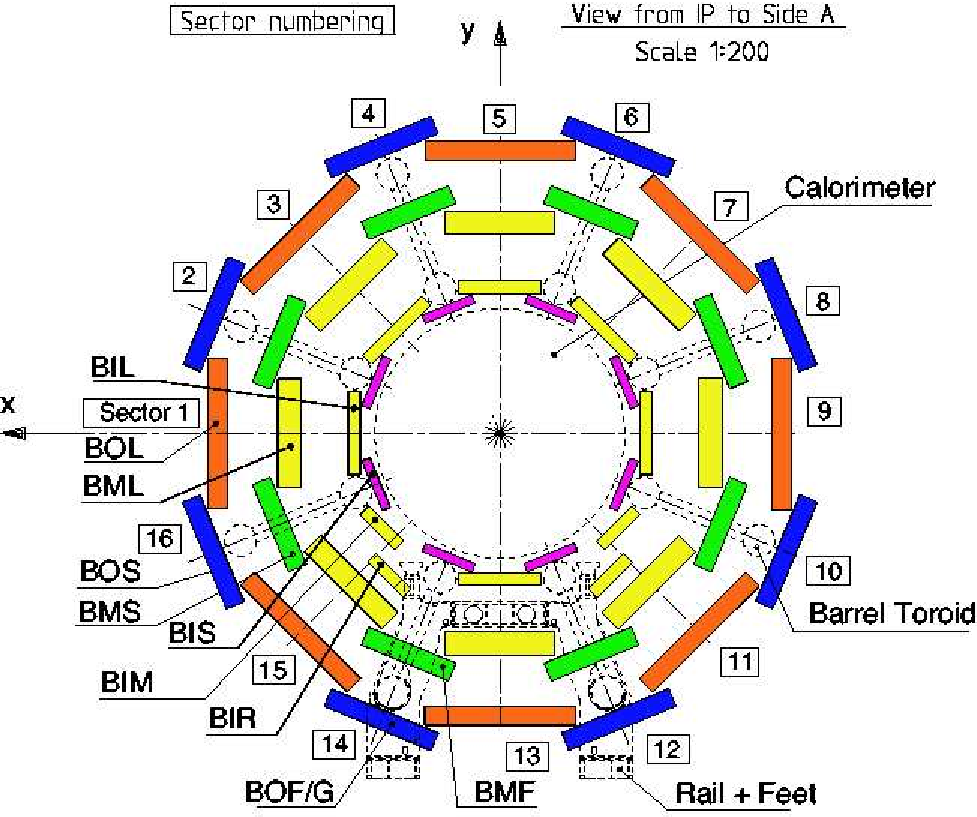
\includegraphics[width=\textwidth]{fig/Muon_sector_numbering.pdf}
      \caption{}
      \label{fig:muon_xy}
  \end{subfigure}
 \begin{subfigure}[b]{0.45\textwidth}
      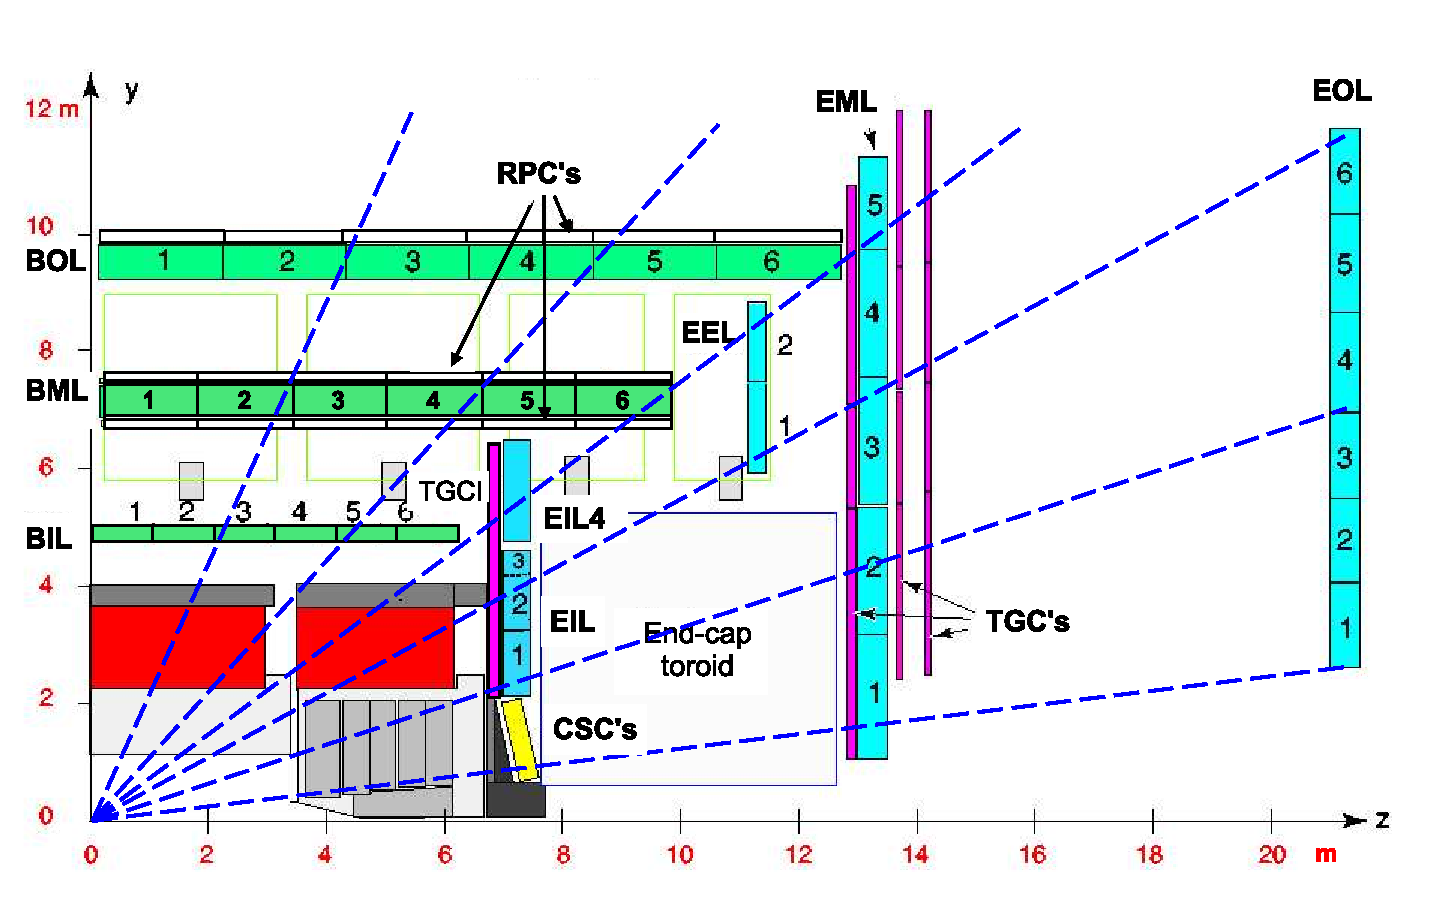
\includegraphics[width=\textwidth]{fig/Muon_rz_large_sect_6.pdf}
      \caption{}
      \label{fig:muon_rz}
  \end{subfigure}
\caption{(a) 与束流垂直方向($x-y$平面)的$\mu$子谱仪布局,它有三层同心圆柱,每层包含8个大室和8个小室,最外层半径大约为20米。(b) $y-z$平面的$\mu$子谱仪布局}
%,Cross-section of the muon system in a plane containing the beam axis (bending plane). Infinite-momentum muons would propagate along straight trajectories which are illustrated by the dashed lines and typically traverse three muon stations.} 
\label{fig:muon_overview}
\end{center}
\end{figure}

\subsection{触发和数据采集系统}
%由于数据存储容量和速率的限制,LHC每秒产生大量的事例必须经过实时筛选和在线触发\cite{Artz_2015},最终只有一小部分被记录。
%当前的ATLAS触发系统包括基于硬件使用来自量能器和$\mu$子系统粗略测量的触发(L1),以及基于软件的高级触发(HLT)。L1将事件发生率(这指bunch-crossing)从40 MHz降低到100 kHz,HLT进一步将其降低到1 kHz的平均记录速率\cite{Artz_2015}。ATLAS数据采集(TDAQ)系统的示意图如图\ref{fig:ATLAS_TDAQ}所示。
%L1触发系统执行初始事件选择并接受100 kHz速率的事件。它经过优化,可以快速做出决策。它联合量能器和MS的信息搜索高能量轻子,光子和喷注。电子和光子触发基于EM量能器中的能量沉积,这
%受限于EM本身分段。
%在强子量能器中,使用滑动窗口算法得到的触发元素形成的簇射最终构建候选喷注。
%一个触发元素是$0.2\times0.2(\eta-\phi)$单元格的总能量沉积,滑动窗口算法会在$4\times4$区域在特定阈值之上检查总$E_{T}$。$\mu$子触发基于触发室若干层着火点重合。
LHC束团间距为25 ns,那么束团碰撞率为40 MHz,质子非弹性散射率接近1 GHz,平均pileup数为23.7,考虑到电子读出系统和数据存储能力的限制,ATLAS仅能处理并存储极少数的事例。
ATLAS触发和数据采集系统(TDAQ)\cite{Aaboud2017}是探测器的基本组成部分,它负责决定是否为以后的离线研究保存事件。

TDAQ有两级:基于硬件的使事例率降低至100 kHz的Level-1触发器(L1),以及基于软件的高级触发器(HLT)系统。HLT使用4万个CPU,并在一次LHC注入期间以1 kHz的平均速率选择事件,这是离线计算模型和存储可以处理的最大值。

L1触发器包括中央触发处理器(CTP),它处理来自L1量能器(L1Calo)和L1~$\mu$子(L1Muon)触发子系统的输入。L1Calo直接从量能器获取信息。L1Muon利用桶部($\abseta<1.0$)RPC和$1.0<\abseta<2.4$区的TGC进行测量。
为了应对更高的事件发生率并有效地选择感兴趣的物理事件,在2016年一个称为L1拓扑处理器(L1Topo)\cite{Simioni:2014nha}的新元素添加到L1中。L1Topo系统从L1Calo和L1Muon获取信息,可以计算不变质量等物理变量以用于L1决策。
由于L1电子设备的延迟为2.5 $\mu\text{s}$,CTP也应用预防性死时间,设置L1连续两次接受决策之间的最短时间以避免重叠读出窗口,并限制在给定束团对撞数目内L1接受决策数以避免前端缓冲区溢出。

在L1触发接受之后,HLT使用更细粒度的量能器信息,来自MS的精确测量以及来自ID的径迹信息来处理事件。为了最大限度地提高效率,HLT软件经过调整,使算法和选择尽可能接近离线重建。
HLT接受的事件最终存储在磁盘上,并导出到CERN计算中心进行离线重建。根据需要,HLT可以处理来自L1处识别的感兴趣区域(RoI)或来自完整探测器的信息。ATLAS触发系统的完整方案如图~\ref{fig:ATLAS_TDAQ}所示。
\begin{figure}[h]
\begin{center}
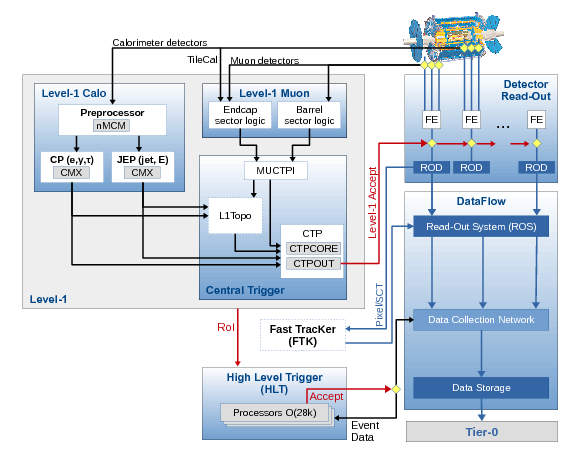
\includegraphics[width=0.75\textwidth]{fig/content_tdaq_figures_tdaq-run2-schematic.png}
\caption{ATLAS TDAQ系统\cite{Aaboud2017},图中着重标注触发相关部分。L1Topo与FTK正在研究,并未包括本文的结果中。} \label{fig:ATLAS_TDAQ}
\end{center}
\end{figure}

L1和HLT的触发决策根本上是由物理分析决定的,不同物理分析处理不同的物理对象,
而所有这些物理对象归纳起来则给出所谓的触发菜单。菜单中的主要触发器涵盖了各种ATLAS物理搜索所需的所有信号,包括电子、$\mu$子、光子、$\tau$轻子、喷注和丢失能量(MET)。
触发菜单组成和触发阈值针对若干亮度范围进行了优化,以便最大化实验的物理输出并且满足ATLAS探测器读出速率和带宽限制。
许多ATLAS分析的主要特征信号,包括$hh\rightarrow 4W$搜索,是电子或者$\mu$子。 因此,在事件中需要存在至少一个$\pt>$25 GeV轻子的触发占据可用带宽的很大一部分,如图\ref{fig:Trigger_singlelepton}所示。
\begin{figure}[h]
\begin{center}
\begin{subfigure}[b]{\textwidth}
\centering
   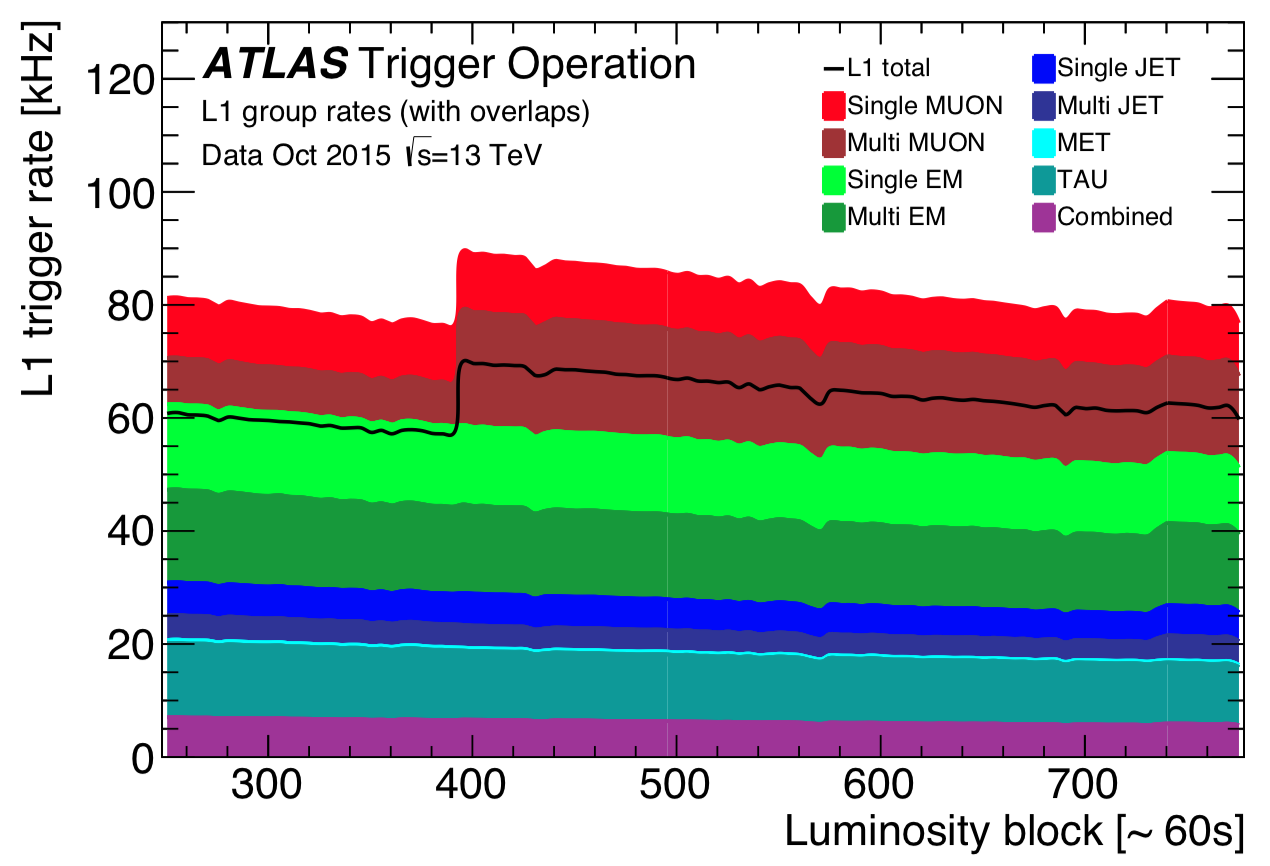
\includegraphics[width=0.75\textwidth]{fig/content_menu_figures_Time_L1GroupRate_Stack.png}
   \caption{}
  \label{fig:L1_menu_rates}
  \end{subfigure}
 \begin{subfigure}[b]{\textwidth}
 \centering
  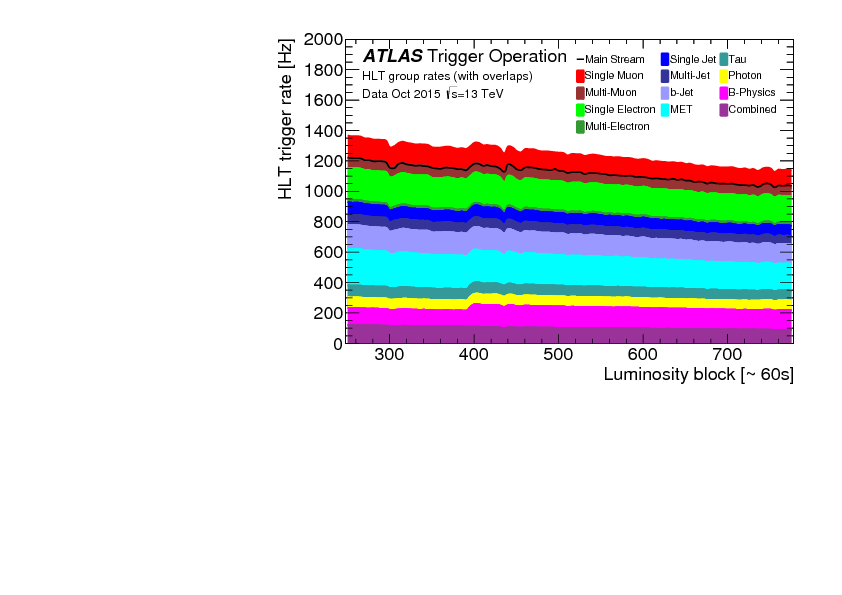
\includegraphics[width=0.75\textwidth]{fig/content_menu_figures_Time_HLTGroupRate_Stack.png}
   \caption{}
   \label{fig:HLT_menu_rates}
  \end{subfigure}
\caption{2015年LHC一次注入(fill)时的L1(a)和HLT(b)的各种信号组的触发率,此次注入最高亮度为$4.5\times10^{33}\text{cm}^{-2}\text{s}^{-1}$。因为各种信号类别之间有重叠,所以他们的触发率之和高于总的触发率(黑色实线),Multi-object触发项包含在b-jets与tau信号组中。亮度区间400之后的触发率增长是因为移除了B-physics prescaling。Combined触发组包含不同的触发信号,比如电子与$\mu$子, $\tau$, jets或者MET。\cite{Aaboud2017}} \label{fig:Trigger_singlelepton}
\end{center}
\end{figure}
